\documentclass[A4paper, 11pt]{article}
\usepackage[slovene]{babel}
\usepackage[utf8]{inputenc}
\usepackage{array}
\usepackage{amsfonts}
\usepackage{amsmath}
\usepackage{pifont}
\usepackage{theorem}
\usepackage{authblk}
\usepackage{url}

\usepackage{graphicx}
\usepackage{subcaption}
\graphicspath{ {slike/} }

\title{Problem simetrične diskretne verižnice z liho mnogo členki}
\author{Klementina Pirc}
\affil{Fakulteta za matematiko in fiziko \\ Oddelek za matematiko}
\date{julij 2020}

\newtheorem{definicija}{Definicija}
\theorembodyfont{\mdseries}
\newtheorem{zgled}{Zgled}

\newcommand{\cmark}{\ding{51}}
\newcommand{\xmark}{\ding{55}}

\begin{document}

\begin{titlepage} 

\maketitle
\thispagestyle{empty}
	
\end{titlepage}


% OPIS PROBLEMA

\section{Opis problema}

Imamo diskretno verižnico, to je verižnico sestavljeno iz palic, katerih dolžino in maso poznamo. Konca verižnice pritrdimo v točki $T1$ in $T2$. Zanima nas oblika verižnice, ki pri tem nastane, torej želimo izračunati koordinate stičišč palic. Vemo, da na verižnico deluje sila gravitacije, zato bo njena oblika takšna, da bo potencialna energija verižnice najmanjša možna. 

V nadaljevanju bom predstavila postopek rešitve za poseben primer diskretne verižnice in sicer za simetrično diskretno verižnico z liho mnogo členki. Simetričnost pomeni, da sta točki $T1$ in $T2$ na enaki višini, ter da so dolžine in mase palic simetrične glede na sredinsko palico. Oglejmo si sedaj še matematično formulacijo problema.

Diskretna verižnica je sestavljena iz $2p+1$ palic, kjer je $p \in \mathbb{N}$. Poznamo dolžine in mase palic, torej $L_i$ in $M_i$ za $i=1, \ldots, 2p+1$. Želimo izračunati koordinate krajišč palic $(x_i,y_i)$ za $i=1, \ldots, 2p$, $(x_0,y_0)$ in $(x_{2p+1},y_{2p+1})$ pa že poznamo, saj sta to obesišči verižnice, torej $T1$ in $T2$. Zaradi simetričnosti velja $y_0 = y_{2p+1}$ ter $L_{2p+2-i} = L_i$ in $M_{2p+2-i} = M_i$ za $i=1, \ldots, p$.

\begin{figure}[h]
\begin{subfigure}{.5\textwidth}
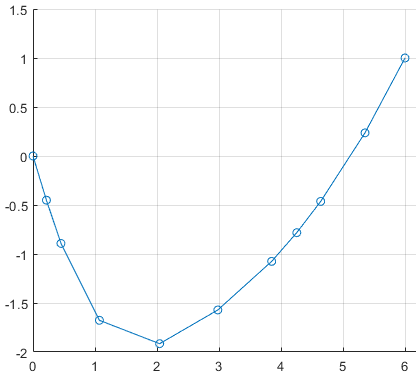
\includegraphics[scale=0.5]{diskretna_premaknjena}
\caption{Diskretna verižnica}
\end{subfigure}
\begin{subfigure}{.5\textwidth}
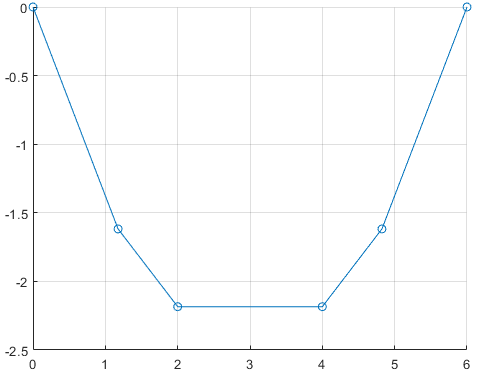
\includegraphics[scale=0.5]{simetricna_liha}
\caption{Simetrična diskretna verižnica z liho mnogo členki}
\end{subfigure}
\end{figure}

\hspace{0.5cm}

% REŠEVANJE

\section{Reševanje problema}

Prvi del postopka je enak kot pri rešitvi za splošno diskretno verižnico, le da že upoštevamo liho število palic in pišemo $2p+1$ namesto $n+1$. 
Minimizirati želimo potencialno energijo verižnice oziroma sistema homogenih palic. Potencialno energijo posamezne palice opišemo z enačbo
\[ W_i = \frac{1}{2} \cdot M_i \cdot g \cdot (y_{i-1} + y_i) \quad za \quad i=1, \ldots, 2p+1 \]
torej je potencialna energija celotne verižnice enaka
\[ W = \sum_{i=1}^{2p+1} W_i = \sum_{i=1}^{2p+1} \frac{1}{2} \cdot M_i \cdot g \cdot (y_{i-1} + y_i) \]
$g$ je gravitacijska konstanta in ne vpliva na minimum potencialne energije, zato jo lahko izpustimo in obravnavamo le funkcijo
\[ F(x,y) = \sum_{i=1}^{2p+1} \frac{1}{2} \cdot M_i \cdot (y_{i-1} + y_i) \]
Za iskane točke $(x_i,y_i)$ velja še Pitagorov izrek $(x_i - x_{i-1})^2 + (y_i - y_{i-1})^2 = L_i ^2$, kar pomeni, da iščemo vezani ekstrem. 

Uporabimo Lagrangeovo metodo in problem prevedemo na reševanje (nevezanega) ekstrema funkcije
\[ G(x,y,\lambda) = \sum_{i=1}^{2p+1} \frac{1}{2} M_i (y_{i-1} + y_i) + \lambda_i ((x_i - x_{i-1})^2 + (y_i - y_{i-1})^2 - L_i ^2) \]
$G$ parcialno odvajamo po $x_i, y_i$ za $i=1, \ldots, 2p$ ter po $\lambda_i$ za $i=1, \ldots, 2p+1$.

\[ \frac{\partial G}{\partial x_i} = 2\lambda_i (x_i - x_{i-1}) - 2\lambda_{i+1} (x_{i+1} - x_i) \qquad i=1, \ldots, 2p \]
\[ \frac{\partial G}{\partial y_i} = \frac{1}{2} (M_i + M_{i+1}) + 2\lambda_i (y_i - y_{i-1}) - 2\lambda_{i+1} (y_{i+1} - y_i) \qquad  i=1, \ldots, 2p \]
\[ \frac{\partial G}{\partial \lambda_i} = (x_i - x_{i-1})^2 + (y_i - y_{i-1})^2 - L_i ^2 \qquad i=1, \ldots, 2p+1 \]
Za preglednejši zapis uvedemo 
\begin{equation}
\begin{split}
\xi_i = x_i - x_{i-1} \qquad i=1, \ldots, 2p+1 \\
\eta_i = y_i - y_{i-1} \qquad i=1, \ldots, 2p+1 \\
\mu_i = \frac{M_i + M_{i+1}}{2} \qquad i=1, \ldots, 2p
\end{split}
\end{equation}
odvode enačimo z 0, še malo uredimo in dobimo $6p+1$ enačb

\begin{equation}
\lambda_i \xi_i - \lambda_{i+1} \xi_{i+1} = 0 \qquad i=1, \ldots, 2p 
\end{equation}

\begin{equation}
\lambda_i \eta_i - \lambda_{i+1} \eta_{i+1} = - \frac{1}{2} \mu_i \qquad i=1, \ldots, 2p 
\end{equation}

\begin{equation}
\xi_i ^2 + \eta_i ^2 = L_i ^2 \qquad i=1, \ldots, 2p+1 
\end{equation}

Zgornji sistem enačb v primeru splošne diskretne verižnice preoblikujemo v sistem dveh enačb za 2 neznanki. V našem primeru pa bomo zaradi lihega števila členov in simetričnosti verižnice sistem lahko preoblikovali kar v eno enačbo z eno neznanko. 

Iz enačbe (2) sledi spodnja enakost
\[ \lambda_i \xi_i = - \frac{1}{2u} \qquad oziroma \qquad \lambda_i = - \frac{1}{2u \xi_i} \qquad i=1, \ldots, 2p  \]
$u$ je konstanta, ki jo bomo določili kasneje. Enakost vstavimo v enačbo (3) in dobimo
\[ \frac{\eta_i}{2u \xi_i} - \frac{\eta_{i+1}}{2u \xi_{i+1}} = \frac{1}{2} \mu_i \qquad i=1, \ldots, 2p \]
Z nekaj preurejanja pridemo do rekurzivne enačbe
\[ \frac{\eta_{i+1}}{\xi_{i+1}} =  \frac{\eta_i}{\xi_i} - u \mu_i \]
Ker enaka enačba velja tudi za $\frac{\eta_i}{\xi_i}, \frac{\eta_{i-1}}{\xi_{i-1}}$ itd., dobimo naslednjo zvezo
\begin{equation}
\begin{split}
\frac{\eta_{i}}{\xi_{i}} & =  \frac{\eta_{i-1}}{\xi_{i-1}} - u \mu_{i-1}  \\
                                               & =  \frac{\eta_{i-2}}{\xi_{i-2}} - u \mu_{i-2} - u \mu_{i-1}  \\
                                               & = \ldots  \\
                                               & = \frac{\eta_1}{\xi_1} - u (\mu_1 - \mu_2 - \ldots - \mu_{i-1})  \\
                                               & = \frac{\eta_1}{\xi_1} - u \sum_{j=1}^{i-1} \mu_j
\end{split}
\end{equation}

Označimo $v = \frac{\eta_1}{\xi_1}$. Pri splošni diskretni verižnici smo sistem enačb izrazili z $v$ in $u$ ter nato poiskali ustrezna približka. V našem primeru, pa lahko zaradi posebnih lastnosti verižnice, $v$ zapišemo kot izraz odvisen od $u$ in celoten sistem sistem izrazimo le z $u$.

Diskretna verižnica ima liho število palic, ki se paroma ujemajo glede na sredinsko palico, tako po masi, kot tudi po dolžini. Ker sta tudi obesišči na enaki višini, iz vseh teh lastnosti sledi, da je sredinska palica vzporedna $x$ osi. V matematičnem jeziku to pomeni
\begin{equation}
x_{p+1} - x_p = \xi_{p+1} = L_{p+1} \qquad in \qquad y_{p+1} - y_p = \eta_{p+1} = 0
\end{equation}
kjer sta $(x_p,y_p), (x_{p+1}, y_{p+1})$ krajišči sredinske palice.

Enačbi iz (6) sedaj uporabimo v (5) in dobimo
\[ \frac{\eta_{p+1}}{\xi_{p+1}} =  \frac{\eta_1}{\xi_1} - u \sum_{j=1}^{p} \mu_j \]
\[ 0 =  \frac{\eta_1}{\xi_1} - u \sum_{j=1}^{p} \mu_j \]
\[ \frac{\eta_1}{\xi_1} = v =  u \sum_{j=1}^{p} \mu_j \]

Sedaj lahko enačbo (5) zapišemo kot
\begin{equation} 
\frac{\eta_{i}}{\xi_{i}} = u \left (\sum_{j=1}^{p} \mu_j - \sum_{j=1}^{i-1} \mu_j \right )
\end{equation}
jo vstavimo v enačbo (4), ter izrazimo $\xi_i$
\[ \xi_i ^2 + \xi_i ^ 2 u^2 \left (\sum_{j=1}^{p} \mu_j - \sum_{j=1}^{i-1} \mu_j \right ) ^2 = L_i ^2 \]
\begin{equation}
\xi_i = \frac{L_i}{\sqrt{1 + u^2 \left (\sum_{j=1}^{p} \mu_j - \sum_{j=1}^{i-1} \mu_j \right ) ^2}} \qquad i = 1, \ldots, 2p+1
\end{equation}
Izbrali smo pozitivno rešitev za $\xi_i$, saj verižnico opazujemo od levega obesišča proti desnemu in so zato $\xi_i$ pozitivni.

Enačbe (2),(3),(4) smo uspešno izrazili le z $u$, kar pomeni, da moramo sedaj najti ustrezen približek zanj. Nato $u$ vstavimo v enačbo (8), ki nam poda vrednosti za vse $\xi_i$. Le-te uporabimo v enačbi (7) in dobimo še vrednosti za $\eta_i$. S tem smo našli vrednosti vseh koordinat krajišč palic, saj iz definicije $\xi_i$ in $\eta_i$ sledi 
\begin{equation}
\begin{split}
x_i = x_0 + \sum_{j=1}^{i} \xi_j \qquad i = 1, \ldots, 2p+1 \\
y_i = y_0 + \sum_{j=1}^{i} \eta_j \qquad i = 1, \ldots, 2p+1
\end{split}
\end{equation}

Približek za $u$ bomo poiskali z Newtonovo metodo. To je iteracijska metoda za iskanje ničle funkcije, ki dobro deluje pri iskanju ničle prve stopnje s primernim začetnim približkom $x_0$. Do novega približka pridemo s formulo
\[ x_{n+1} = x_n - \frac{f(x_n)}{f'(x_n)} \]
kjer je $f$ funkcija, katere ničlo iščemo, $f'$ pa njen odvod. 

Preden lahko uporabimo Newtonovo metodo, moramo definirati funkcijo $U(u)$, katere približek za ničlo bo naš približek za $u$.
Če upoštevamo, da je $\xi_i = x_i - x_{i-1}$, vidimo da lahko zapišemo
\[ U(u) = \sum_{i=1}^{2p+1} \xi_i - x_{2p+1} + x_0 = 0 \]
in $u$ res nastopa v zgornji funkciji, saj smo $\xi_i$ izrazili z njim. Za preglednejši zapis definiramo še 
\begin{equation}
w_i = u \nu_i \qquad i=1, \ldots, 2p+1
\end{equation}
\begin{equation}
\nu_i = \left ( \sum_{j=1}^{p} \mu_j - \sum_{j=1}^{i-1} \mu_j \right ) \qquad i=1, \ldots, 2p+1
\end{equation}
in dobimo
\begin{equation}
U(u) =  \sum_{i=1}^{2p+1} L_i (1 + w_i ^2) ^ {-\frac{1}{2}} - x_{2p+1} + x_0
\end{equation}
Odvod $U$ pa je
\begin{equation}
U'(u) = \frac{dU}{du} (u) = - \sum_{i=1}^{2p+1} L_i (1 + w_i ^2) ^ {-\frac{3}{2}} w_i \nu_i 
\end{equation}
(12), (13) sedaj vstavimo v predpis za Newtonovo metodo in dobimo iteracijsko formulo s katero izračunamo približek za $u$. Izbrati moramo le še ustrezen začetni približek $u_0$. Iteracijo zaključimo, ko je razlika zadnjih dveh izračunanih približkov manjša od tolerance, ki smo jo izbrali.
\[ u_{n+1} = u_n - \frac{U(u_n)}{U'(u_n)} \]

% IMPLEMENTACIJA

\section{Implementacija}

Poženemo skripto \textit{simetricna\_liha\_ver.m}, v kateri smo navedli:
\begin{itemize}
\item obesišči verižnice $(x_0,y_0)$,$(x_{2p+1},y_{2p+1})$ v obliki $zac = [x_0 \  x_{2p+1};\  y_0 \  y_{2p+1}]$, 
\item vrstico dolžin palic $L = [L_1 \  L_2 \ \ldots \ L_{2p+1}]$,
\item vrstico mas palic $M = [M_1 \ M_2 \ \ldots \ L_{2p+1}]$.
\end{itemize}
Najprej kličemo funkcijo \textit{risi\_veriznica(zac,L,M)}, ki nam vrne matriko iskanih koordinat koncev palic, hkrati pa še izriše obliko verižnice. Sedaj dani verižnici s funkcijo \textit{razpolovi\_palice(L,M)} vse palice razdelimo na dva enaka dela in tako dobimo podatke $L1, M1$ za novo diskretno verižnico. Z \textit{risi\_veriznica(zac,L1,M1)} poračunamo in izrišemo še njeno obliko. Nazadnje izvršimo še funkcijo \textit{animacija(X,X1)}, ki sprejme koordinate obeh verižnic in prikaže, kako so se posamezne točke premaknile.

Prvotna verižnica ima liho mnogo členov, zato problem rešujemo po zgoraj opisanem postopku. Z razpolavljanjem palic pa dobimo verižnico s sodo mnogo členi in za reševanje uporabimo splošno rešitev, ki smo jo implementirali na vajah. Funkcija \textit{risi\_veriznica} se na podlagi dolžine vektorja $L$ odloči, kateri postopek bo uporabljen.

V primeru lihega števila definira začetni približek $u_0$ in pokliče funkcijo \textit{ver\_u($u_0$,zac,L,M)}. Le-ta najprej izračuna vektor $\mu$ s členi $\mu_i$ iz enačbe (1) ter vektor \textit{vsote\_mi} delnih vsot iz enačbe (11). S pomočjo \textit{sistem\_u(u,zac,L,vsote\_mi)} dobimo predpis za funkcijo $U(u)$ (enačba (12)), potem pa poiščemo približek za njeno ničlo z Newtonovo metodo. Dobljen približek $u$ uporabimo v vektorjih \textit{ksi} in \textit{eta}, katerih elementi so definirani v enačbah (8) in (7). Nazadnje uporabimo še predpisa iz enačbe (9) in dobimo vektorja $x$,$y$ s koordinatami krajišč palic podane verižnice.


% REZULTATI

\section{Rezultati} 
Oglejmo si nekaj primerov simetričnih diskretnih verižnic z lihim številom členov in pripadajočo verižnico, ki jo dobimo z razpolavljanjem palic. \\
\\
zac = [0 6; 0 0], \quad L = [2 1 2 1 2], \quad M = [1 0.5 1 0.5 1]
\begin{figure}[h]
\begin{subfigure}{.5\textwidth}
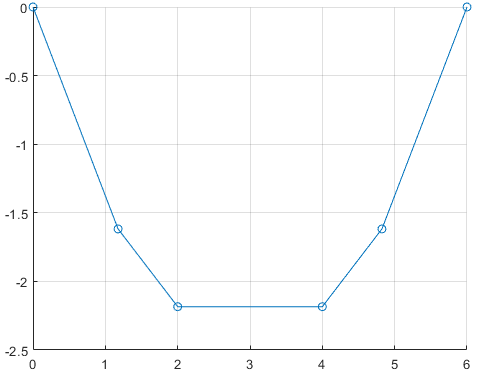
\includegraphics[scale=0.5]{simetricna_liha}
\end{subfigure}
\begin{subfigure}{.5\textwidth}
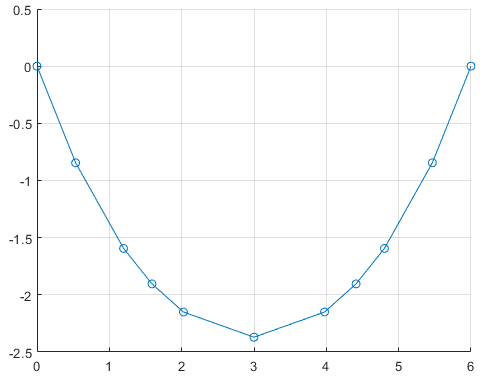
\includegraphics[scale=0.5]{prepolovljena}
\end{subfigure}
\end{figure}
\begin{figure}[h]
\centering
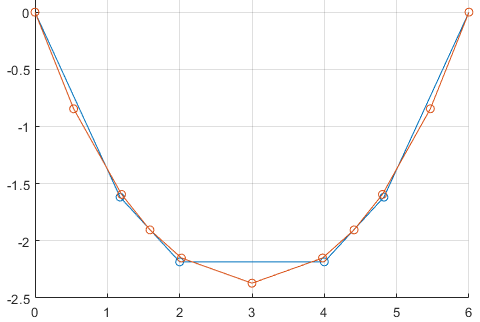
\includegraphics[scale=0.8]{liha_in_soda}
\end{figure}

\newpage

zac = [0 3; 0 0], \quad L = [5 2 5], \quad M = [2 0.5 2]
\begin{figure}[h]
\begin{subfigure}{.5\textwidth}
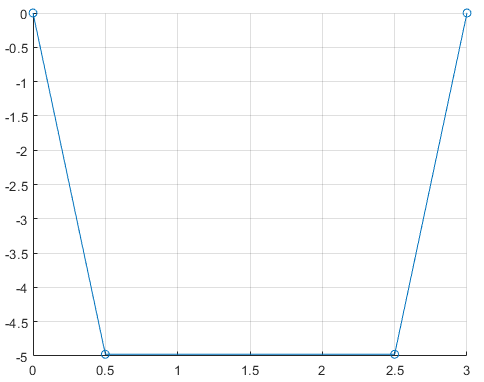
\includegraphics[scale=0.5]{simetricna_liha_2}
\end{subfigure}
\begin{subfigure}{.5\textwidth}
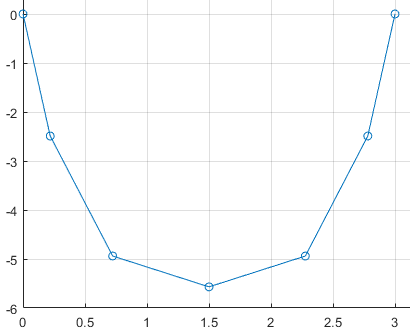
\includegraphics[scale=0.5]{prepolovljena_2}
\end{subfigure}
\end{figure}
\begin{figure}[h]
\centering
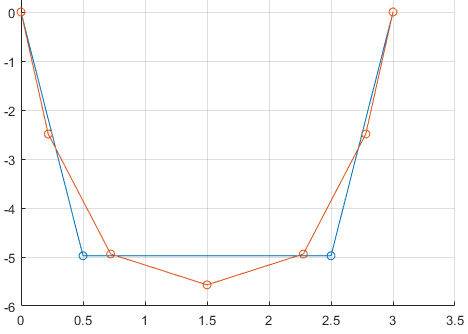
\includegraphics[scale=0.8]{liha_in_soda_2}
\end{figure}

\newpage

zac = [0 10; 0 0], \quad L = [4 3 2 1 2 3 4], \quad M = [3 2 1 1 1 2 3]
\begin{figure}[h]
\begin{subfigure}{.5\textwidth}
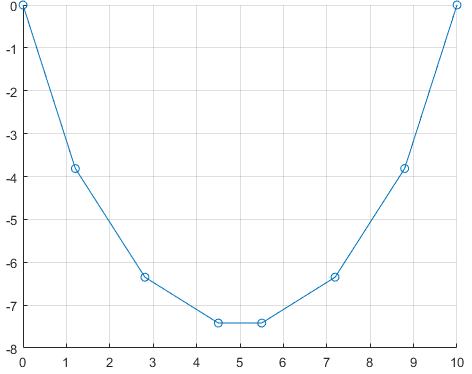
\includegraphics[scale=0.5]{simetricna_liha_3}
\end{subfigure}
\begin{subfigure}{.5\textwidth}
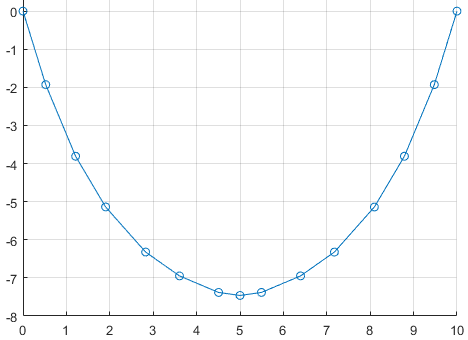
\includegraphics[scale=0.5]{prepolovljena_3}
\end{subfigure}
\end{figure}
\begin{figure}[h]
\centering
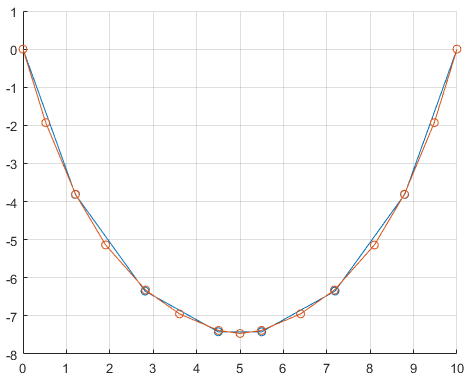
\includegraphics[scale=0.8]{liha_in_soda_3}
\end{figure}


% LITERATURA

\begin{thebibliography}{9}
\bibitem{veriznica}
	E. Zakrajšek, \emph{Verižnica} (1999) od 6 do 10.
	Dostopno na spletni učilnici FMF 2019/2020 predmeta Matematično modeliranje [22. 7. 2020]
\bibitem{zapiski}
	Zapiski s predavanj predmeta Matematično modeliranje.
\end{thebibliography}

\end{document}


